%!TEX root = ../Thesis.tex
\chapter{Preface}
\vspace*{1cm}
{\centering
\sffamily
This dissertation is presented by\\[3mm]
{\large Jesper S{\"o}ren Dramsch}\\[3mm]
to the\\[3mm]
{\large Department of Physics}\\[3mm]
in partial fulfilment of the requirements for the degree of\\[3mm]
{\large Doctor of Philosophy (Ph.D.)}\\[3mm]
in the subject of\\[3mm]
{\large Physics}

\vfill

    \thesislocation{}, November 14\textsuperscript{th}, 2019\\[1cm]
\begin{flushright}
    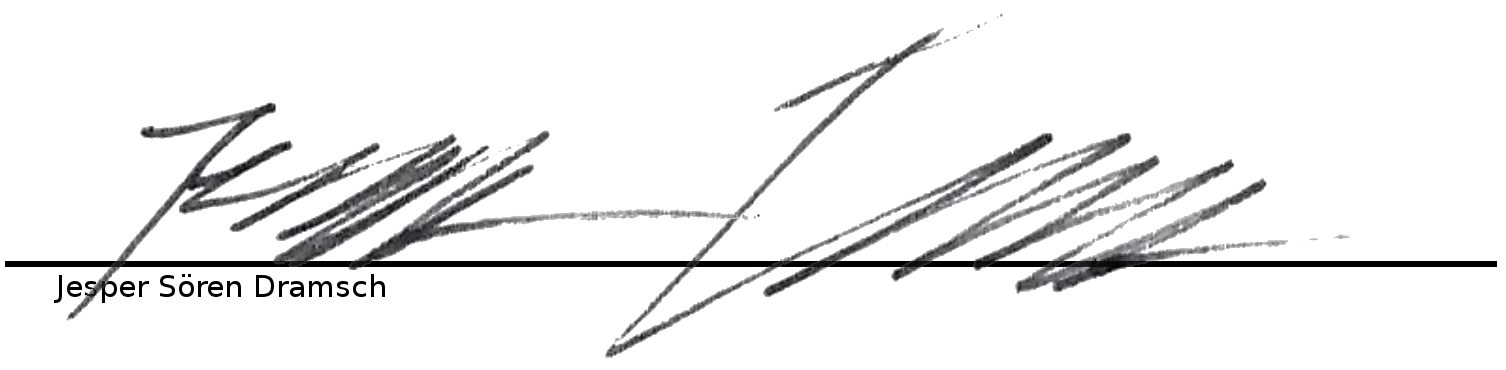
\includegraphics[width=0.45\textwidth]{graphics/Unterschrift.png}\\[1cm]
\end{flushright}
}
\clearpage
\newpage
\vspace*{3cm}
{\sffamily
\begin{tabular}{ll}
Ph.D. Thesis & \\[1mm]
University: & Technical University of Denmark (DTU)  \\[1mm]
Department: & Department of Physics / Centre for Oil and Gas -- DTU \\[1mm]
Author: & Jesper S{\"o}ren Dramsch \\[1mm]
Title: & Machine Learning in 4D Seismic Data Analysis\\[1mm]
       &Deep Neural Networks in Geophysics \\[1mm]
Principal Advisor: \hspace{1cm} & Mikael L{\"u}thje \\[1mm]
Co-Advisor: & Anders Nymark Christensen (DTU Compute) \\[1mm]
External Advisor: & Colin MacBeth (Heriot-Watt University, UK) \\[1mm]
Submitted: & 2019-11-14 
\end{tabular}
}